% !TEX root = ../../../main.tex
% 来源：中学数学实验教材·第一册（代数）
% 章节：因式分解与余式定理 / 辗转相除法
% 原始文件：5.tex，行 2547-2567
% 类型：tikz
% ---
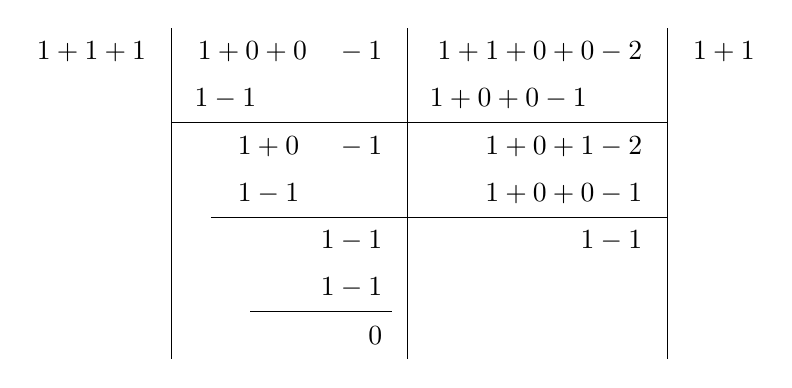
\begin{tikzpicture}[yscale=.6]
\foreach \y/\ytext in {6/1+0+0\quad -1  ,5/1-1\qquad\qquad \;\;  ,4/ 1+0\quad\; -1  , 3/ 1-1\qquad \quad , 2/1-1  , 1/1-1 ,0/ 0}
{
    \node at (-.2,\y)[left]{$\ytext$};
}

\foreach \y/\ytext in {6/1+1+0+0-2  ,5/1+0+0-1\qquad ,4/ 1+0+1-2  , 3/ 1+0+0-1  , 2/\boxed{1-1}}
{
    \node at (3.1,\y)[left]{$\ytext$};
}
\foreach \x in {-3,0,3.3}
{
    \draw(\x,6.5)--(\x, -.5);
}

\draw(-3,4.5)--(3.3,4.5);
\draw(-2.5,2.5)--(3.3,2.5);
\draw(-2,.5)--(-.2,.5);
\node at (-3.2,6)[left]{$1+1+1$};
\node at (3.5,6)[right]{$1+1$};
\end{tikzpicture}
